\documentclass[tikz,border=6pt]{standalone}
\usepackage{amsmath,amssymb}
\definecolor{inM}{RGB}{31,94,165}\definecolor{inC}{RGB}{214,96,33}
\tikzset{
  m/.style={circle,inner sep=0pt,minimum size=9pt,ball color=inM!85,draw=inM!60!black,line width=0.3pt},
  c/.style={circle,inner sep=0pt,minimum size=9pt,ball color=inC!90,draw=inC!60!black,line width=0.3pt},
  lab/.style={font=\small,fill=white,fill opacity=0.85,text opacity=1,inner sep=1.2pt,rounded corners=1pt},
  e/.style={line width=0.75pt,black!55},
  ec/.style={line width=1.5pt,inC!80!black}}
\begin{document}
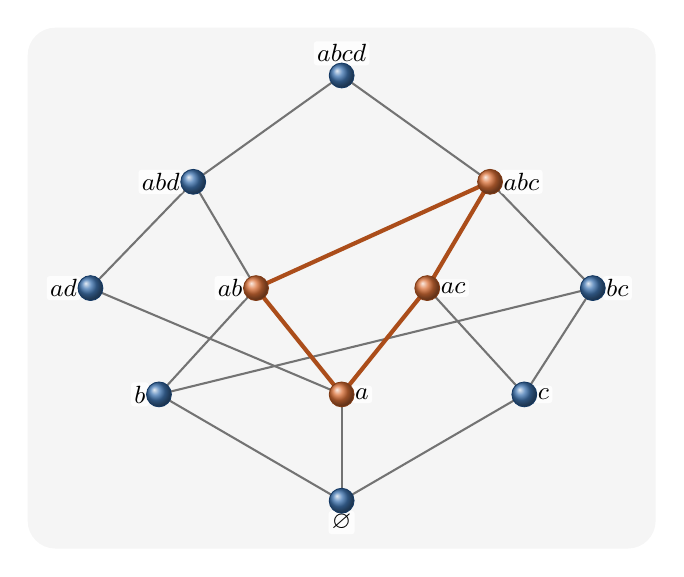
\begin{tikzpicture}[x=1.45cm,y=1.35cm]
\fill[black!4,rounded corners=10pt] (-2.75,-0.45) rectangle (2.75,4.45);
\coordinate (0) at (0,0);
\coordinate (b) at (-1.6,1); \coordinate (a) at (0,1); \coordinate (cc) at (1.6,1);
\coordinate (ad) at (-2.2,2); \coordinate (ab) at (-0.75,2); \coordinate (ac) at (0.75,2); \coordinate (bc) at (2.2,2);
\coordinate (abd) at (-1.3,3); \coordinate (abc) at (1.3,3);
\coordinate (X) at (0,4);
\foreach \u/\v in {0/b,0/a,0/cc,b/bc,cc/bc,a/ad,ad/abd,ab/abd,bc/abc,abd/X,abc/X,b/ab,cc/ac}
  \draw[e] (\u) -- (\v);
\foreach \u/\v in {a/ab,a/ac,ab/abc,ac/abc}
  \draw[ec] (\u) -- (\v);
\foreach \n/\t/\p in {0/{\varnothing}/below,b/b/left,a/a/right,cc/c/right,ad/ad/left,ab/ab/left,ac/ac/right,bc/bc/right,abd/abd/left,abc/abc/right,X/abcd/above}
  \node[lab,\p=3.5pt] at (\n) {$\t$};
\foreach \n in {0,b,cc,ad,bc,abd,X} \node[m] at (\n) {};
\foreach \n in {a,ab,ac,abc} \node[c] at (\n) {};
\end{tikzpicture}
\end{document}
